\documentclass[12pt,journal]{IEEEtran}
\usepackage[
backend=biber,
style=numeric,
citestyle=numeric]{biblatex}
\addbibresource{citations.bib}
\usepackage{pifont}
\usepackage{caption}
\usepackage{graphicx}
\usepackage{wrapfig,booktabs}
\usepackage{authblk}
\usepackage{hyperref}
\captionsetup{justification=raggedright,singlelinecheck=false}
\providecommand{\keywords}[1]{\textbf{Keywords} #1}
\begin{document}
\title{Capture and Replay Tools in the Field}
\author[1]{Deepa Chhetri}
\author[1]{Brian Pollack}
\affil[1]{Department of Electrical Engineering and Computer Science, Case Western Reserve University}
\maketitle

\begin{abstract}
In GUI applications, a user interacts with the system via graphical interface such as mouse click, scroll, drag, text box etc. There could be large number of possible sequences in which a user can interact. Testing such application means ensuring the correct sequence of interactions resulting in desired output. If this testing is done manually, it could be tedious. Therefore, capture and replay tools came into existence. It  enables the testers to record the entire ineteractive session and replaying it at any later time. By replaying a given log file on a changed version of the application, capture and replay tools thus support fully-automatic regression testing of graphical user interfaces.
\end{abstract}

\keywords\\{GUI testing; capture and replay tools; Reanimator}

\section{Introduction}

\IEEEPARstart{S}{oftware} testing is a process of  evaluating software for its functionality by performing some test cases on an attribute or capability of a program or system and determining that it meets its required results. Testing involves the execution of a software component or system component to evaluate one or more properties of interest. Testing the graphical user interface (GUI) of a software product is important to ensure the quality of the system and therefore to improve the user experience\cite{Nedyalkova:2013:OSC:2494444.2494464}. It not only involves testing the GUI but also the functionality of system. But manual testing the GUI is tedious and time consuming. GUI capture and replay tools were developed as a mechanism for testing the correctness of interactive applications with graphical user interfaces. Using a capture and replay tool, a tester can run an application and record the entire interactive session. The tool records all the user's events, such as the keys pressed or the mouse movements, in a log file called test scripts. Given tets scripts, the tool can then automatically replay the exact same interactive session any number of times without requiring a human user. This helps in early detection of bugs that might lead to system failure and therefore speed up the process of development.
\par
The advantages of using capture and replay tools include saving time by making the process quicker and easier. Capture and replay tools save time by not forcing the developers to hand-code test scripts which would need to be updated each time the application is changed. They also make it simple for testers without significant programming skills to automate their test cases \cite{McMaster:2009:EHF:1547559.1548260}. This means that companies can hire employees dedicated to testing who are not required to know high level programming, therefore lowering testing costs. However, these tools do have some drawbacks. They don't generate test cases automatically, sometimes the recorded test scripts are inefficient and require manual intervention, and the tools know only how to interact with widgets, but they have no idea with which application they are operating \cite{michaelsilverstein2003}. During regression testing, any change to the GUI may cause a test case to break or stop execution of the updated version \cite{McMaster:2009:EHF:1547559.1548260}.
\par
In this paper we compare four capture and replay tools using different criteria. This comparison study will be beneficial to software developers who want to choose a capture and replay tool which would be a good fit for testing their applications. Further we explain how we extended Reanimator, an existing capture and replay tool, and enhanced it by adding functionality that will help web developers effectively run capture and replay tests in the field.
\par
The remainder of this paper is organized as follows: Section 2 discusses previous research regarding the comparison of capture and replay tools; Section 3 summarizes each tool that was used for our comparison; Section 4 decribes the evaluation criteria used to establish the comparison; Section 5 describes the results of our analysis; Section 6 describes our modifications to Reanimator; Section 7 contains a summary of our work.

\section{Literature Review}
Nedyalkova and Bernardino established a comparison of capture and replay tools. They evaluated five open source capture and replay tools: Abbot, Jacareto, JFCUnit, Marathon, and Pounder. The criteria that they used for comparison is divided into two major groups - ``General Characteristics'' and ``Capture/Replay Characteristics''. General characteristics include:
\begin{enumerate}
\item Easy to Install
\item User Interface
\item Easy to Use
\item Easy to Launch Application Under Test (AUT)
\item Documentation
\item Tutorials
\item Examples
\item Programming Skills Required
\end{enumerate}
Capture/Replay Characteristics include:
\begin{enumerate}
\item Text Field - interaction with a JTextField
\item Mouse Move - detection of mouse movements on a component
\item Mouse Drag - detection of mouse drags
\item Mouse Clicks - detection of mouse clicks
\item Component - interaction with a window
\item Scrolling - interaction with the scrollbar of a JTextArea
\item File Dialog - navigating the directories in a JFileChooser
\item Combo Box - selecting an item in a JComboBox
\end{enumerate}
Based on their analysis, Nedyalkova and Bernardino determined that Jacareto is the best tool among the five they evaluated. Jacareto is easy to install, had better documentation, does not require additional programming skills, and supports all capture and replay characteristics except for navigation of dialog box. Jacareto allows the tester to speed up or slow down the replay of the application log, helping make testing more efficient \cite{Nedyalkova:2013:OSC:2494444.2494464}.
\par
Similarly, Rodrigues et al. performed an empirical comparison to evaluate Capture/Replay (CR based) and Model-Based Performance (MBT) testing tools. They studied the effort required (time spent) to use both CR-based and MBT tools. They compared LoadRunner and Visual Studio, both CR-based tools, and the PLeTsPerf MBT tool to create performance test scripts and scenarios to test web applications. LoadRunner is a performance testing tool based on the CR technique that supports scripts generation and execution to test Web-based applications. Visual Studio is an IDE developed by Microsoft to support software design, development and test. PLeTsPerf is a model-based performance testing tool. Rodrigues et al. used used an in-vitro approach, since it refers to the experiment in the laboratory under controlled conditions, addressing a real problem, i.e., the differences in individual effort to create performance test scripts and scenarios using LoadRunner,VisualStudio and PLeTsPerf. They performed the experiment to answer three research questions:
\begin{enumerate}
\item What is the effort to generate a single performance test script and scenario using PLeTsPerf, LoadRunner, and VisualStudio?
\item What is the effort to re-generate performance test scripts and scenarios when using PLeTsPerf, LoadRunner, and VisualStudio?
\item What is the effort to generate a set of performance test scripts and scenarios using PLeTsPerf, LoadRunner, and VisualStudio?
\end{enumerate}
The experiment execution phase was split into three sessions, each composed of three tasks. These tasks were performed using the PLeTsPerf, LoadRunner  and VisualStudio approaches, one for each task, and all tasks should generate an equivalent performance test script as an output. They summarize the results by giving average time spent per treatment to complete each session. They determined that for simple testing tasks the effort of using CR-based tool was less than MBT tool but as the complexity of testing task increases the advantage of using MBT grows significantly \cite{Rodrigues:2014:ECR:2652524.2652587}.
\par
Mugshot is a deterministic capture and replay tool developed by Microsoft. It captures every event that is executed in JavaScript program which can be replayed deterministically at any later time to analyze the sequence of events that might have led to system failure. To capture application activity, it records all sources of nondeterminism. If an application is run again and injected with the same non deterministic events, the program will follow the same execution path that was observed at logging time. It has its client side implemented in JavaScript to easily record logs instead of downloading additional plug-ins. For each new event it captures, it creates a log entry that contains a sequence number and wall clock time. The entry also contains the event type and enough type-specific data to recreate event at play time. Mugshot uses a caching proxy to reproduce the load events in the log \cite{Mickens:2010:MDC:1855711.1855722}. This is the limitation of Mugshot. If an application fetches external contents that does not pass through the proxy, Mugshot cannot guarantee faithful replay of its data or its load time.

\section{Description of Capture and Replay Tools Used}
In this section, we give a short description of capture and replay tools analyzed in this study. We focused on those capture and replay tools that are built for internet applications. Here, we compared four tools $-$ Reanimator, Sahi, Telerik and Selenium IDE:
\subsection{Reanimator}
Reanimator\footnote{https://github.com/WaterfallEngineering/reanimator} captures non-deterministic input to a JavaScript application in a log that can be replayed at a later time. It was originally designed for recording web application crashes in the wild for later debugging. It is inspired by Microsoft’s Mugshot. It is built on JQuery 1.8.3. The code for Reanimator is available on GitHub and is under MIT license. It works only on Firefox. It supports both Windows and Linux platforms.Reanimator consists of a core, which is responsible for capture setup and driving the replay, and one or more plugins, which are responsible for capturing and replaying non-deterministic input. Reanimator ships with plugins for capturing and replaying random numbers, dates, and timer interrupts.

\subsection{Sahi}
Sahi\footnote{http://sahipro.com/} is an Automation testing tool that is used for testing web application. There are two versions of Sahi tool. One is open source and is available on SourceForge. The other, named Sahi Pro, is proprietary and is available on their official website. It has powerful abilities for recording and replaying across browsers; different language drivers for writing test scripts (Java, Ruby); and support for AJAX and highly dynamic web applications. Sahi also supports https and NTLM authentications. It works on Internet Explorer, Firefox and Chrome. It only supports Windows platform. The following figure shows how Sahi fits in a simulated user operation:
\begin{figure}[h!]
 \hfill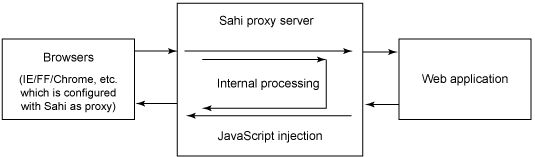
\includegraphics[width=9cm]{figures/sahi.PNG}\hspace*{\fill}
 \caption{Simulated user operation}
 \label{fig}
\end{figure}

\subsection{Telerik}
Telerik Test Studio\footnote{http://www.telerik.com/teststudio} is commercial windows-based software testing tool with Visual Studio plugins. It facilitates web and desktop (GUI) functional testing, performance testing and mobile app testing with Record and Replay features. It supports JavaScript, HTML, ASP.NET, Ajax, Silverlight etc and facilitates quick validations. It works on Internet Explorer, Firefox, Chrome and Safari. It has features like visual storyboard and 3D element selection. It also offers script-lesstest automation for Silverlight applications. Test Studio offers three product versions:
\begin{enumerate}
\item The Functional version performs web and WPF testing and includes the Visual Studio plugin.
\item The Load version performs load testing.
\item The Ultimate version combines Web, Mobile, WPF, Load testing and Test Studio for APIs.
\end{enumerate}

\subsection{Selenium IDE}
Selenium IDE\footnote{http://www.seleniumhq.org/projects/ide/}: Selenium is known as umbrella project that enables web browser testing for all browsers. It is a open source free application supports GUI Testing and web functional testing. It is implemented as a Firefox extension, and allows recording, editing, and debugging tests. It includes the entire Selenium Core which allows easy and quick record and play back tests in the actual environment that they will run in. It supports both Windows and Linux platforms.Selenium IDE supports autocomplete mode when creating tests. This feature serves two purposes:\\
$\bullet$ It helps the tester to enter commands more quickly.\\
$\bullet$ It restricts the user from entering invalid commands.\\

\section{Evaluation of Existing Tools}
The four tools discussed in the previous section were installed on an HP laptop with Intel core i5 processor (2.30 GHz), 4 GB RAM and windows 8.1 operating system with Java 1.8. We installed the tools Sahi, Telerik and Selenium. The code for Reanimator was directly deployed on a web server we manage. Initially, to test these tools (except for Reanimator) a simple online calculator written in Javascript was deployed to one of our webservers. The demo code for Reanimator comes with a simple puzzle game.
\par
The following criteria are used to establish comparison between these tools:\\ \\
\textbf{ \textit{Evaluation for ease of deployment:}}
\begin{enumerate}
\item Easy to install
\item Time required to install
\item User interface
\item Tutorials available
\item Open source
\item Programming skills required
\item Documentation provided
\item Examples provided
\item User interface for developers\\
\end{enumerate}
\textbf{\textit{Evalution for level of detail of measurements:}}
\begin{enumerate}
\item Interaction with text fields
\item Mouse movements
\item Mouse clicks
\item Mouse drags
\item Scrolling
\item Dialog box\\
\end{enumerate}
\textbf{\textit{Additional system information:}}
\begin{enumerate}
\item Size
\item Platforms
\item Browser support
\item Additional features\\
\end{enumerate}

Table 1 shows the comparison between Reanimator, Sahi, Telerik  and Selenium based on criteria for evalution for ease of deployment. Table 2 shows the comparison based on criteria for evalution for level of detail of measurements. Table 3 shows the additiona system information provided with each tool. The symbol \ding{51} means that the tool provides the characteristic which is in evaluation and the symbol \ding{55} means that it doesn’t support it. \\

\begin{figure}[h!]
 \hfill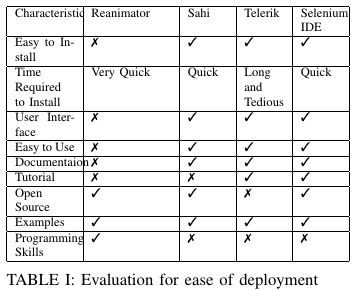
\includegraphics[width=9cm]{figures/table1.PNG}\hspace*{\fill}
\end{figure}
\begin{figure}[h!]
 \hfill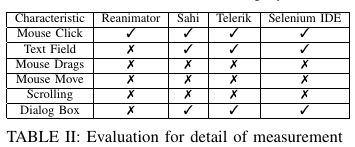
\includegraphics[width=9cm]{figures/table2.PNG}\hspace*{\fill}
\end{figure}

\begin{figure}[h!]
 \hfill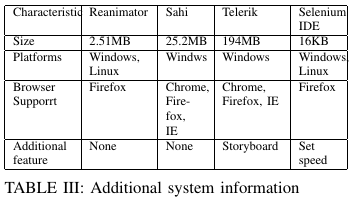
\includegraphics[width=9cm]{figures/table3.PNG}\hspace*{\fill}
\end{figure}


\section{Comparison Analysis}
All of the tools we tested are at least functional: they capture interactive web sessions and successfully play them back at a later time. While taking all criteria into consideration, Sahi performs better overall than the other tools we tested.
\par
Compared to Telerik and Reanimator, Sahi has easier installation. It has strong documentation available online. It does not require any programming skill to use Sahi. Sahi supports Chrome, Firefox and Internet Explorer. Selenium is easiest to install as it comes as firefox plugin. It also provides all the features like Sahi but the greatest setback of selenium is that it can only be used to capture and replay Firefox sessions. It has a great feature that allows the user to set speed to analyse the scenarios. No other tool provides this feature and has their own replay speed. This makes the process of analysis cumbersome if the default speed is very fast or slow. Telerik has a major setback that its installation takes very long (it took us 1 day to install) to finish since it requires lot of dependencies and also its installation process is not very effective. It requires large hard disk space. It has the feature called visual storyboard which gives the snapshot of each scenario recorded by tool. This allows the developer to go to any snapshot. We used the one month free trial version of Telerik and requires to purchase once the trial period expires. Telerik also supports Chrome, Firefox and Internet Explorer. Reanimator is a small capture and replay tool inspired by Mugshot. It requires programming skills since it does not come as ready to use testing tool. It is built on JQuery 1.8.3. It requires programming skills to get Reanimator working.Also it works only on Firefox and Internet Explorer. It does not have any additional feauture.
\par
Later, we talk about modifications we made to Reanimator that make it more functional and easier to use. We compared the four tools, however, as we found them directly from their authors. We did not compare our upgraded version of Reanimator during this test.
\par
Based on the evalution criteria seen in table 1, 2 and 3, we choose Sahi as the best tool among all others.


\section{Extension and Modification of Reanimator}
We forked the original Reanimator GitHub project at \href{https://github.com/brianmpollack/reanimator}{https://github.com/brianmpollack/reanimator}. It took awhile to determine exactly how the original authors built Reanimator, but we were able to understand their work to determine how Reanimator was built.
\subsection{Original Reanimator Code}
Reanimator is built as an extension to JQuery and uses NodeJS to compile the source files. The compile scripts start with JQuery and use Almond to inject the Reanimator codebase. The main driver of Reanimator is contained in the lib/reanimator/core.js file. There is a file in the lib/reanimator/plugins directory which serves as the implementation for each logging feature that Reanimator supports.

\subsection{Issues with Original Code}
The original Reanimator code contained a few runtime and compilation issues, which we fixed before continuing to work with Reanimator.

\subsubsection{Google Chrome}
First, we observed that the precompiled code in the demos did not work in Google Chrome. It appears that the original authors tried to convert DOM objects to JSON. DOM stands for Document Object Model and JavaScript uses DOM Objects to represent the webpage contents.
\par
It is commonly known that JSON does not support circular references, but DOM Objects contain numerous circular references. Some browsers, such as Firefox, will simply proceed with the JSON encoding and will automatically drop the circular references, but other browsers, such as Chrome, will terminate the JavaScript process. We found a simple function that will remove the circular references from the DOM object while converting it to JSON, allowing Reanimator to now be used in any major browser (this fixed Reanimator in our tests with Chrome, Firefox, Safari, Internet Explorer, and Edge).

\subsubsection{File Link Error}
We also found a file error in the included demos. The original Makefile used a symbolic link to link the Reanimator JavaScript code to the demos, rather than copying the files. The symbolic link, however, caused issues both when the code is uploaded to GitHub and even when running locally.
\par
We updated the Makefile to copy the files into the demo folders. While we could have updated the demo code to link to the dist directory of the Reanimator code, we felt that it was important to allow the demos to be self-contained. This would allow a user to copy the contents of a demo folder directly to their server for testing.

\subsection{Uploading Log to Server}
Originally, Reanimator was not very useful to developers in the field. As soon as a user closed his or her browser, any recorded log would be destroyed. To make Reanimator more useful to developers, the main feature we wanted to add was log uploading.

\subsubsection{Client Side}
We refer to the Reanimator JavaScript code as the client side because it is running locally on the web client’s machine. To enable log uploading, we modified the capture function in the core.js file. We added parameters so the user could pass in a boolean to enable uploading, and so the client could pass in a UUID to be associated with the log. A UUID, or Universally Unique Identifier, is a unique ID for the client. Generation and use of UUIDs is outlined in RFC 4122. \cite{p.leachm.meallingr.salz2005}
\par
The client, if log uploading is enabled, will upload the log to an HTTP POST service every five seconds. By default, we programmed Reanimator to POST to a file called reanimator.php in the same directory as the JavaScript file.
\par
We duplicated and extended the original tile game demo to support uploading to a webservice. A user can play the tile game, then can select a list of sessions from a dropdown. After selection, he or she can see any past game that was logged to the server.

\subsubsection{Server Side}
The server can be written any way the developer prefers as long as it accepts HTTP POST requests.
\par
We included a sample HTTP POST web service file in the dist directory of Reanimator. The simple script is written in PHP and will upload the logs to a MySQL database for retrieval later. It will overwrite any old logs with the same UUID.
\par
We also included a sample database configuration file with the uploading tile game demo. Because a developer should know how to setup a simple web service and MySQL server, we do not feel the need to explain them in detail.

\section{Future Additions to Reanimator}
In the future, we recommend adding more features to Reanimator. We believe that it is useful to developers after our additions, but could be improved further.

\subsection{Developer Interface on Playback}
We propose creating a developer interface, or developer portal. It would provide a user friendly way for developers to organize and replay their captured sessions. The interface could include a play/pause button, and let the developer choose the speed to play back the session.
\par
Because this does not add any core functionality, but rather an improved user experience, we recognize that it would help developers but we did not choose to implement it during our Reanimator extension/proof of usefulness test.

\subsection{Synchronize Only Changes}
Our demonstration implementation will upload the user's log every five seconds. The server code will simply overwrite the log data for that user in the database when it receives new data. This practice is fine for demo purposes and for small websites, but is obviously not scalable to large websites. We propose uploading only the changes of the log to the server.
\par
To ensure that data is not lost, we could allow the server to respond to the POST request to tell the client if the log upload was successful. The client would keep track of successful log pushes and would know if it needs to retry or if it can upload a new section of the log.
\par
This modification would appear small to each client, but would be a huge difference to large websites which could potentially be receiving many log pushes at the same time.

\subsection{Smaller Upload Size}
The log files that Reanimator generates are large relative to the usefull information that they contain. The files contain every piece of information about the layout of the webpage. We propose modifying the way that logs are stored. There will be one initial log with the entire DOM, but subsequent events will simply be a changelog of the original log file.
\par
This would make the entire log smaller, allowing for smaller uploads and less memory used at the client.
\par
It is important to note that this solution is different from the previous suggestion (synchronizing only the changes). The entire log would be much smaller, as it would only contain the changes to the original log file. We can combine this with the previous suggestion to further minimize the overhead of Reanimator.

\section{Conclusion}
In our study, we compared four capture and replay tools, namely Reanimator, Sahi, Telerik and Selenium. The goal of this study was to determine the best tool among these which has best overall performance. These tools were compared on different criteria to find out which tool has reliable capture and replay capabilities without requiring too much human efforts. After evaluating each one of the tools, we came to a conclusion that the tool that best satisfies our requirements is Sahi. This tool stood out from rest of the tools as it has best overall performance. Therefore, we can say that Sahi can be easily adapted by any developer to test their GUI application. We also worked on Reanimator to enhance it by additing new functionalities to it. We enabled it to work on Chrome. We ...{to be added by Brian}




\printbibliography

\end{document}
